% Final presentation: 10 minutes + 5 minutes Q&A. Compile from presentations/:
% lualatex presentation.tex (twice). See CLAUDE.md.
% Main part: about 7 min of work and results, then 3 min of novelty, code, team, verification,
% learnings, challenges, limitations. Backup slides after "Thank you" for questions.
% Content: Stage 2 report, Stage 3 report (v5), and the ltp tool from Stage 4.
\documentclass[aspectratio=169,14pt]{beamer}
\usepackage[T1]{fontenc}
\usepackage{lmodern}
\usepackage{booktabs}
\usepackage{amsmath}
\usepackage{adjustbox}
\usepackage{appendixnumberbeamer}
\usepackage{tikz}
\usetikzlibrary{arrows.meta,positioning}
\graphicspath{{../experiments/}{figures/}}

% ---- standard Beamer theme, orange ---------------------------------
\usetheme{Madrid}
\definecolor{orangetheme}{HTML}{E8710A}
\definecolor{accent}{HTML}{C2570C}
\definecolor{muted}{HTML}{6B7280}
\definecolor{soft}{HTML}{FDEFE3}
\usecolortheme[named=orangetheme]{structure}
\setbeamercolor{alerted text}{fg=accent}
\setbeamertemplate{navigation symbols}{}
\setbeamertemplate{itemize items}[circle]
\setbeamertemplate{blocks}[rounded][shadow=false]
\setbeamerfont{frametitle}{series=\bfseries}
% small white logo icon at the right end of every frame title bar
\addtobeamertemplate{frametitle}{}{%
  \begin{tikzpicture}[remember picture,overlay]
    \node[anchor=north east,inner sep=0pt] at ([xshift=-0.25cm,yshift=-0.12cm]current page.north east)
      {
\includegraphics[height=0.75cm]{tapasense_icon_white.png}};
  \end{tikzpicture}}

\newcommand{\sub}[1]{{\color{muted}\small #1}}
\newcommand{\fig}[2][0.74]{\centering\includegraphics[height=#1\textheight,width=\textwidth,keepaspectratio]{#2}}
\newcommand{\us}{\,$\mu$s}
% link to a backup slide, shown small in the corner of a main slide
\newcommand{\backup}[2]{\hfill\hyperlink{#1}{\beamerbutton{#2}}}

\title[TapaSense]{Lightweight Temperature Predictor}
\author[Kurien, Mase]{Ethan Bobby Kurien \and Kaivalya Mase}
\date{}

\begin{document}

% =====================================================================
% MAIN PART 1 (about 7 minutes): what we did and the results
% =====================================================================
\begin{frame}[plain]
  \centering
  
\includegraphics[width=0.62\textwidth]{tapasense_lockup.png}\\[1.2em]
  {\color{black!85}\Large\bfseries Lightweight Temperature Predictor}\\[0.3em]
  {\color{muted} Calibrate once per floorplan, then predict in microseconds}\\[1.6em]
  Ethan Bobby Kurien \qquad Kaivalya Mase
\end{frame}

% ---------------------------------------------------------------------
\begin{frame}{The problem}
  \fig[0.36]{P0-3_block_vs_grid/results/maps_128.png}\\[-0.2em]
  \centering\sub{HotSpot grid at nominal power, one floorplan per style.}\\[0.3em]
  \raggedright
  \begin{itemize}
    \item Thermal management needs core temperatures \alert{every millisecond}.
    \item HotSpot (chip thermal simulator): accurate, but \alert{0.24\,s} per answer.
    \item Task: calibrate once, then predict steady and transient temperatures.
  \end{itemize}
\end{frame}

% ---------------------------------------------------------------------
\begin{frame}{Key observation: HotSpot is linear}
  \begin{columns}[c]
    \column{0.50\textwidth}
      \centering
      \adjincludegraphics[trim={0 0 {.5\width} 0},clip,height=0.66\textheight]{P0-2_linearity/results/transient_linearity.png}
    \column{0.48\textwidth}
      Power doubles, rise doubles.\\
      Rises from different cores add.\\[0.6em]
      So in steady state:
      \[
        \boxed{\;T = T_\text{amb} + G\,P\;}
      \]
      $G_{ij}$ = rise of block $i$\\ per watt in core $j$.
  \end{columns}
\end{frame}

% ---------------------------------------------------------------------
\begin{frame}{Our approach: two stages}
  \centering
  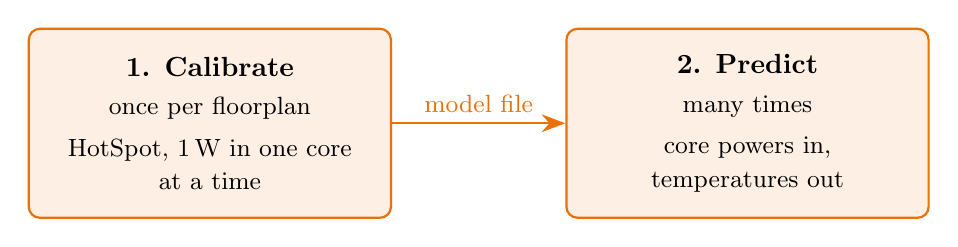
\begin{tikzpicture}[
      box/.style={draw=orangetheme,fill=soft,rounded corners=4pt,thick,
                  minimum width=4.6cm,minimum height=2.4cm,align=center},
      >={Stealth[length=3mm]}]
    \node[box] (cal) {\textbf{1. Calibrate}\\[0.2em]\small once per floorplan\\[0.3em]
                      \small HotSpot, 1\,W in one core\\ \small at a time};
    \node[box,right=2.2cm of cal] (pred) {\textbf{2. Predict}\\[0.2em]\small many times\\[0.3em]
                      \small core powers in,\\ \small temperatures out};
    \draw[->,thick,orangetheme] (cal) -- node[above]{\small model file} (pred);
  \end{tikzpicture}\\[1em]
  \begin{itemize}
    \item Calibration: a few planned HotSpot runs.
    \item Prediction: use the calibrated coefficients, without HotSpot.
  \end{itemize}
\end{frame}

% ---------------------------------------------------------------------
\begin{frame}{Models we tried}
  \begin{columns}[T]
    \column{0.48\textwidth}
      \begin{block}{Steady state}
        {\small Power held constant: where do the temperatures settle?}
        \begin{itemize}
          \item S0: power blurring \backup{b-s0}{more}
          \item \alert{\textbf{S1: influence matrix}}
          \item S2: low-rank $G$ \backup{b-s2}{more}
        \end{itemize}
      \end{block}
    \column{0.48\textwidth}
      \begin{block}{Transient}
        {\small Power changes every ms: temperature over time.}
        \begin{itemize}
          \item T1: one time constant \backup{b-t1}{more}
          \item T2: fitted to one trace \backup{b-t2}{more}
          \item \alert{\textbf{T3: sum of exponentials}}
        \end{itemize}
      \end{block}
  \end{columns}
  \vspace{0.8em}
  \centering \alert{\textbf{Bold}}: the models we kept.
\end{frame}

% ---------------------------------------------------------------------
\begin{frame}{Steady state: the influence matrix S1}
  \begin{columns}[c]
    \column{0.48\textwidth}
      $G_{ij}$: rise of block $i$ with 1\,W in core $j$:
      \[
        G_{ij} = T_i(\text{1\,W in core } j) - T_\text{amb}
      \]
      Then predict $T = T_\text{amb} + G\,P$.\\[0.6em]
      One HotSpot run per core, about \alert{4\,s} in total.\\
      Exact, because HotSpot is linear.
    \column{0.50\textwidth}
      \centering
      \adjincludegraphics[trim={0 {.5\height} {.5\width} 0},clip,height=0.58\textheight]{P1-1_step_calibration/results/G_heatmaps_stage2.png}\\
      \sub{Little cores heat themselves most.}
  \end{columns}
\end{frame}

% ---------------------------------------------------------------------
\begin{frame}{Is calibration really needed?}
  \begin{columns}[c]
    \column{0.54\textwidth}
      \fig[0.74]{P1-3_is_calibration_needed/results/error_by_method_stage2.png}
    \column{0.44\textwidth}
      \alert{\textbf{Yes.}} Without runs on the chip:\\[0.4em]
      \small
      \begin{tabular}{@{}l c@{}}
        \toprule
        Method & Mean error \\
        \midrule
        \textbf{S1, calibrated} & \textbf{0.000007\,K} \\
        S0 power blurring & 0.76\,K \\
        Borrow $G$, same style & 1.11\,K \\
        Borrow $G$, other style & 2.79\,K \\
        \bottomrule
      \end{tabular}
  \end{columns}
\end{frame}

% ---------------------------------------------------------------------
\begin{frame}{S1 against HotSpot}
  \centering
  \adjincludegraphics[trim={{.247\width} {.288\height} {.282\width} {.487\height}},clip,height=0.42\textheight]{extended_validation/results/heatmaps.png}\\
  \sub{Left: HotSpot block averages. Right: S1 prediction.}\\[0.4em]
  \small
  \begin{tabular}{@{}c c c c@{}}
    \toprule
    Worst error & Time & Size & vs HotSpot \\
    \midrule
    \alert{0.00003\,K} & \alert{2.6\us} & \alert{928\,B} & \alert{91{,}000$\times$} faster \\
    \bottomrule
  \end{tabular}\\[0.3em]
  \sub{Tested on 24 floorplans, 302 power vectors each.}
\end{frame}

% ---------------------------------------------------------------------
\begin{frame}{Hot spots: S1-hot-max}
  \begin{columns}[c]
    \column{0.34\textwidth}
      \centering
      \adjincludegraphics[trim={{.745\width} 0 0 0},clip,height=0.56\textheight]{P0-3_block_vs_grid/results/maps_128.png}\\
      \sub{HotSpot grid}
    \column{0.64\textwidth}
      \begin{itemize}
        \item HotSpot divides the floorplan into a $64\times64$ grid of cells $q$.
        \item Hottest cell: 3.3--4\,K above the core average.
      \end{itemize}
      Same runs give $G$ for every cell; take the max:
      \[
        T_\text{hot}(c) = T_\text{amb} + \max_{q\,\in\,c}\; \sum_j G^\text{cell}_{qj} P_j
      \]
      Mean error: \alert{0.000007\,K} (core average: 2.73\,K).
      \backup{b-hot}{more}
  \end{columns}
\end{frame}

% ---------------------------------------------------------------------
\begin{frame}{Transient: T3, sum of exponentials}
  \textbf{Calibrate:} switch on 1\,W in core $j$, record the rise $s_{ij}(t)$ of core $i$.
  \[
    s_{ij}(t) \approx \sum_{m=1}^{M} a_{ijm}\,\bigl(1 - e^{-t/\tau_m}\bigr),
    \qquad \sum_m a_{ijm} = G_{ij}
  \]
  \begin{itemize}
    \item $\tau_m$: $M$ time constants.
    \item $a_{ijm}$: how much of the heating happens at each speed.
    \item Weights add up to $G_{ij}$: exact in steady state.
  \end{itemize}
  \textbf{Predict:} by linearity, add up the responses to every power change.
  \backup{b-t3}{more}
\end{frame}

% ---------------------------------------------------------------------
\begin{frame}{T3 against HotSpot step responses}
  \fig[0.56]{P1-1_step_calibration/results/step_response_fits_stage3.png}\\[0.3em]
  1\,W switched on in one core.\\
  T3 with $M=4$ follows HotSpot; one time constant (T1) cannot.
\end{frame}

% ---------------------------------------------------------------------
\begin{frame}{Transient models compared}
  \centering
  \begin{tabular}{@{}l c c c c@{}}
    \toprule
    Model & Mean & Worst & Time/step & Size \\
    \midrule
    T1 one time constant & 7.25\,K & 14.6\,K & 1.5\us & 1.0\,kB \\
    T2 fitted to one trace & 0.19\,K & 0.57\,K & 5.4\us & 6.2\,kB \\
    \textbf{T3, $M=4$} & \textbf{0.090\,K} & \textbf{0.30\,K} & \textbf{3.1\us} & \textbf{3.7\,kB} \\
    \bottomrule
  \end{tabular}\\[0.8em]
  \sub{Test traces from a cold chip, 24 floorplans.}
  \backup{b-m}{choosing $M$}
\end{frame}

% ---------------------------------------------------------------------
\begin{frame}{Does it work on chips we never saw?}
  \fig[0.42]{extended_validation/results/transient_check.png}\\[-0.1em]
  \centering\sub{Hottest core of one new floorplan per style: T3 (red dashed) on HotSpot (black).}\\[0.4em]
  \small
  \begin{tabular}{@{}l c c@{}}
    \toprule
    & T3 mean & T3 worst \\
    \midrule
    24 floorplans (development) & 0.090\,K & 0.30\,K \\
    52 new generated floorplans & 0.091\,K & 0.34\,K \\
    \bottomrule
  \end{tabular}
\end{frame}

% ---------------------------------------------------------------------
\begin{frame}[fragile]{The tool: \texttt{ltp}}
  Both stages from the command line or Python, only NumPy needed.
  \vspace{0.4em}
  \footnotesize
\begin{verbatim}
python3 -m src.ltp calibrate s4_fp001 -o model.npz
python3 -m src.ltp transient model.npz --ptrace in.ptrace -o out.ttrace
$ python3 -m src.ltp steady model.npz --power 20,20,8,8,8,8,8,8
Core_0  Core_1  Core_2  Core_3  Core_4  Core_5  Core_6  Core_7
66.313  67.214  68.344  67.488  69.297  68.614  68.760  67.769
\end{verbatim}
  \normalsize
  \vspace{0.4em}
  \begin{itemize}
    \item Reads the given \texttt{.ptrace} files, writes HotSpot-style \texttt{.ttrace}.
    \item \texttt{bench} checks a model against fresh HotSpot runs.
  \end{itemize}
\end{frame}

% ---------------------------------------------------------------------
\begin{frame}{Results against our targets}
  \centering
  \begin{tabular}{@{}l l c c@{}}
    \toprule
    & Metric & Target & Achieved \\
    \midrule
    Steady & mean error & $\le$ 0.1\,K & \alert{0.000006\,K} \\
           & peak error & $\le$ 0.2\,K & \alert{0.00003\,K} \\
           & time & $\le$ 20\us & \alert{2.6\us} \\
           & size & $\le$ 5\,kB & \alert{928\,B} \\
    \midrule
    Transient & mean error & $\le$ 0.5\,K & \alert{0.09\,K} \\
              & worst error & $\le$ 1\,K & \alert{0.30\,K} \\
    \bottomrule
  \end{tabular}
\end{frame}

% =====================================================================
% MAIN PART 2 (about 3 minutes)
% =====================================================================
\begin{frame}{What is new in our work}
  \begin{itemize}
    \item \alert{Exact} steady predictor, \alert{91{,}000$\times$ faster} than HotSpot, from one run per core.
    \item Shown that calibration is \alert{needed}: no shortcut comes close.
    \item Exact hot spots inside cores from the \alert{same runs}.
    \item Transient model: 3.7\,kB, exact in steady state.
    \item Leakage: added as extra power, exact again in 3 iterations.
    \item Tested on \alert{52 floorplans} the models never saw.
    \item Packaged as a tool: \texttt{ltp}.
  \end{itemize}
\end{frame}

% ---------------------------------------------------------------------
\begin{frame}{Code and team}
  \small
  \begin{block}{Ethan \hfill $\approx$ 1{,}500 lines}
    HotSpot runner and patches, linearity, steady-state models, S1-hot-max, leakage.
  \end{block}
  \begin{block}{Kaivalya \hfill $\approx$ 2{,}900 lines}
    Generated floorplans, transient models (T1, T2, T3), calibration-needed study,
    packaging into \texttt{ltp}.
  \end{block}
  \begin{block}{Both \hfill $\approx$ 1{,}650 lines}
    Floorplan and power tooling, other experiments, reports.
  \end{block}
  \centering\normalsize \alert{Total: about 6{,}100 lines}
\end{frame}

% ---------------------------------------------------------------------
\begin{frame}{Verification}
  \begin{columns}[T]
    \column{0.52\textwidth}
      \textbf{Approach}
      \begin{itemize}
        \item Final check on 52 new floorplans.
        \item Stress tests beyond normal use.
        \item Unit tests for the tool.
      \end{itemize}
    \column{0.46\textwidth}
      \textbf{Test cases}\\[0.3em]
      \small
      \begin{tabular}{@{}l r@{}}
        \toprule
        Steady test runs & 7{,}248 \\
        Calibration-free tests & 6{,}946 \\
        Hot-spot test runs & 1{,}380 \\
        Transient floorplans & 24 + 52 \\
        Unit tests (\texttt{ltp}) & 7 \\
        \bottomrule
      \end{tabular}
  \end{columns}
  \backup{b-robust}{robustness}
\end{frame}

% ---------------------------------------------------------------------
\begin{frame}{Learnings and challenges}
  \begin{columns}[T]
    \column{0.50\textwidth}
      \begin{block}{Key learnings}
        \begin{itemize}
          \item HotSpot is linear: a matrix can be exact.
          \item Borrowing $G$ does worse than calibration.
          \item More than one time constant is required.
          \item Averages hide hot spots.
        \end{itemize}
      \end{block}
    \column{0.46\textwidth}
      \begin{block}{Challenges}
        \begin{itemize}
          \item HotSpot prints 0.01\,K, our errors are $10^{-5}$\,K: patched it.
          \item Long transient runs were slow: we cached HotSpot's matrix factorisation, 29$\times$ faster.
        \end{itemize}
      \end{block}
  \end{columns}
\end{frame}

% ---------------------------------------------------------------------
\begin{frame}{Limitations}
  \begin{itemize}
    \item All results are against HotSpot, not real silicon.
    \item A new heat sink needs recalibration (old model 4.4--8.5\,K off).
    \item Leakage handled in steady state only; HotSpot has no transient leakage.
  \end{itemize}
\end{frame}

% ---------------------------------------------------------------------
\begin{frame}[plain]
  \centering\vfill
  
\includegraphics[width=0.45\textwidth]{tapasense_lockup.png}\\[1.6em]
  {\bfseries\LARGE Thank you}
  \vfill
\end{frame}

% =====================================================================
% BACKUP SLIDES (for questions)
% =====================================================================
\appendix

\begin{frame}{Backup slides}
  \begin{columns}[T]
    \column{0.48\textwidth}
      \textbf{Steady state}
      \begin{itemize}
        \item \hyperlink{b-s0}{S0: power blurring}
        \item \hyperlink{b-s2}{S2: low-rank $G$}
        \item \hyperlink{b-hot}{Hot spots in detail}
        \item \hyperlink{b-leak}{Leakage}
      \end{itemize}
    \column{0.48\textwidth}
      \textbf{Transient}
      \begin{itemize}
        \item \hyperlink{b-t1}{T1: one time constant}
        \item \hyperlink{b-t2}{T2: fitted to one trace}
        \item \hyperlink{b-t3}{T3 in detail}
        \item \hyperlink{b-m}{Choosing $M$}
        \item \hyperlink{b-trace}{T3 on a test trace}
        \item \hyperlink{b-robust}{Robustness}
      \end{itemize}
  \end{columns}
\end{frame}

% ---------------------------------------------------------------------
\begin{frame}[label=b-s0]{S0: power blurring (no calibration)}
  \begin{columns}[c]
    \column{0.44\textwidth}
      \fig[0.45]{P1-3_is_calibration_needed/results/s0_kernel.png}
    \column{0.54\textwidth}
      \begin{itemize}
        \item One HotSpot run, 1\,W source on a large die: kernel $K(r)$.
        \item New chip: spread each core's 1\,W over its cells, add up the kernel to get $G$.
        \item No runs on the new chip.
      \end{itemize}
      \vspace{0.4em}
      Result: \alert{0.76\,K} mean, 5.2\,K worst.
  \end{columns}
\end{frame}

% ---------------------------------------------------------------------
\begin{frame}[label=b-s2]{S2: can $G$ be smaller?}
  Keep only the largest parts of $G$ (low rank).\\[0.6em]
  \centering\small
  \begin{tabular}{@{}l l c c@{}}
    \toprule
    Chip & Model & Size & Worst error \\
    \midrule
    8 cores & \textbf{full S1} & \textbf{928\,B} & \textbf{0.00003\,K} \\
            & low rank, $r=2$ & 360\,B & 12.1\,K \\
    \midrule
    64 cores & \textbf{full S1} & \textbf{32.8\,kB} & \textbf{0.00002\,K} \\
             & low rank, $r=32$ & 32.8\,kB & 3.3\,K \\
    \bottomrule
  \end{tabular}\\[0.8em]
  \normalsize
  Heat spreads locally, so $G$ is mostly diagonal.\\ Low rank loses that information.
\end{frame}

% ---------------------------------------------------------------------
\begin{frame}[label=b-hot]{Hot spots in detail}
  \[
    T_\text{hot}(c) = T_\text{amb} + \max_{q\,\in\,c}\; \sum_j G^\text{cell}_{qj} P_j
  \]
  \centering\small
  \begin{tabular}{@{}l c c c@{}}
    \toprule
    Peak model & Size & Mean & Worst \\
    \midrule
    Core average & 512\,B & 2.73\,K & 8.96\,K \\
    \textbf{S1-hot-max, all cells} & \textbf{115\,kB} & \textbf{0.000007\,K} & \textbf{0.00003\,K} \\
    \quad 32-bit & 57\,kB & 0.000007\,K & 0.00003\,K \\
    Coarse grid $32\times32$ & 29\,kB & 0.14\,K & 2.8\,K \\
    Coarse grid $16\times16$ & 7.2\,kB & 0.47\,K & 4.7\,K \\
    Low rank, $r=2$ & 29\,kB & 3.4\,K & 11.4\,K \\
    \bottomrule
  \end{tabular}\\[0.3em]
  Dropping cells that can never be the hottest keeps it exact and smaller.
\end{frame}

% ---------------------------------------------------------------------
\begin{frame}[label=b-leak]{Leakage}
  Hot chips leak more power, which breaks linearity.\\[0.4em]
  Fix: add leakage as extra power and repeat
  \[
    T^{(k+1)} = T_\text{amb} + G\,\bigl(P + P_\text{leak}(T^{(k)})\bigr)
  \]
  \centering\small
  \begin{tabular}{@{}l c c@{}}
    \toprule
    & Worst error & Time \\
    \midrule
    S1 alone & 0.08--0.10\,K & 2.6\us \\
    \textbf{S1 + loop (3 iterations)} & \textbf{1--2$\times10^{-5}$\,K} & \textbf{22--25\us} \\
    \bottomrule
  \end{tabular}\\[0.4em]
  \normalsize\sub{Steady state only: HotSpot has no transient leakage.}
\end{frame}

% ---------------------------------------------------------------------
\begin{frame}[label=b-t1]{T1: one time constant}
  Each core moves part of the way to its S1 value every step:
  \[
    x_i[k+1] = a_i\, x_i[k] + (1-a_i)\,(G\,P[k])_i,
    \qquad a_i = e^{-\Delta t/\tau_i}
  \]
  \begin{itemize}
    \item One $\tau_i$ per core, fitted to the step responses.
    \item Cannot follow 1\,ms and 8\,s at once.
  \end{itemize}
  \vspace{0.4em}
  \centering Result: \alert{7.25\,K} mean, 14.6\,K worst.
\end{frame}

% ---------------------------------------------------------------------
\begin{frame}[label=b-t2]{T2: fitted to one long trace (ARX)}
  Next temperature from past temperatures and powers:
  \[
    x[k] = A_1 x[k-1] + A_2 x[k-2] + B_0 P[k] + B_1 P[k-1]
  \]
  \begin{itemize}
    \item Fitted to one recorded 60\,s HotSpot trace.
    \item Every core switches between random power levels, 1\,ms to 5\,s phases.
  \end{itemize}
  \vspace{0.4em}
  \centering Result: \alert{0.19\,K} mean, 0.57\,K worst. Needs a long trace.
\end{frame}

% ---------------------------------------------------------------------
\begin{frame}[label=b-t3]{T3 in detail}
  \[
    s_{ij}(t) \approx \sum_{m=1}^{M} a_{ijm}\,\bigl(1 - e^{-t/\tau_m}\bigr),
    \qquad \sum_m a_{ijm} = G_{ij}
  \]
  \begin{itemize}
    \item $s_{ij}(t)$: rise of core $i$ after 1\,W is switched on in core $j$.
    \item $\tau_m$: the same for every pair (chip and package).
    \item $a_{ijm}$: how much of the heating happens at each speed.
    \item Weights add up to $G$: exact in steady state.
    \item With $M=6$: $\tau \approx$ 1\,ms, 3\,ms, 26\,ms, 89\,ms, 0.56\,s, 8.1\,s.
  \end{itemize}
\end{frame}

% ---------------------------------------------------------------------
\begin{frame}[label=b-m]{Choosing $M$}
  \begin{columns}[c]
    \column{0.60\textwidth}
      \fig[0.80]{P3-3_pareto/results/pareto_transient_report.png}
    \column{0.38\textwidth}\small
      \begin{tabular}{@{}l c c@{}}
        \toprule
        T3 & Worst & Size \\
        \midrule
        $M=2$ & 2.9\,K & 1.9\,kB \\
        $M=3$ & 1.1\,K & 2.8\,kB \\
        \textbf{$M=4$} & \textbf{0.30\,K} & \textbf{3.7\,kB} \\
        $M=6$ & 0.13\,K & 5.6\,kB \\
        \bottomrule
      \end{tabular}\\[0.8em]
      \normalsize
      Red line: best accuracy for each size. Changing $M$ trades size for accuracy.
  \end{columns}
\end{frame}

% ---------------------------------------------------------------------
\begin{frame}[label=b-trace]{T3 on a test trace}
  \begin{columns}[c]
    \column{0.64\textwidth}
      \fig[0.82]{P3-1_transient_predictor/results/trace_example.png}
    \column{0.34\textwidth}
      T3 (green) closely follows HotSpot (black).\\[1em]
      T1 (blue) is several kelvin off.
  \end{columns}
\end{frame}

% ---------------------------------------------------------------------
\begin{frame}[label=b-robust]{Robustness}
  \centering\small
  \begin{tabular}{@{}l c l@{}}
    \toprule
    Test & Worst error & Verdict \\
    \midrule
    Normal trace (reference) & 0.32\,K & \\
    Transient at 2$\times$ power & 0.64\,K & fine \\
    Bursty power, every 1--5\,ms & 0.44\,K & fine \\
    Warm start & 0.27\,K & fine \\
    \midrule
    New ambient, $T_\text{amb}$ updated & 0.00002\,K & no recalibration \\
    Heat sink changed, old model & 4.4--8.5\,K & recalibrate \\
    Heat sink changed, recalibrated & 0.00001--0.00002\,K & fine \\
    \bottomrule
  \end{tabular}\\[1em]
  \normalsize
  The coefficients belong to the chip \alert{and} its cooling.
\end{frame}

\end{document}
